%!TEX root=paper/thesis.tex
\section{Evaluation}\label{sec:det_evaluation}

We evaluate our system on the multi-class, multi-label detection task, as previously described.
Each detection episode takes an image and outputs detections with associated times, based on the order of actions taken.
We evaluate on a popular detection challenge task: the PASCAL VOC 2007 dataset \cite{pascal-voc-2010}.
This datasets exhibits a rather modest amount of class co-occurrence: the ``person'' class is highly likely to occur, and less than $10\%$ of the images have more than two classes.

We learn weights on the training and validation sets, and run our policy on all images in the testing set.
The final evaluation pools all detections up to a certain time, and computes their multi-class AP per image, averaging over all images.
This is done for different times to plot the AP vs. Time curve over the whole dataset.
Our method of averaging per-image performance follows \cite{Desai2009}.

For the detector actions, we use one-vs-all cascaded deformable part-model detectors on a HOG featurization of the image \cite{Felzenszwalb-CVPR-2010}, with linear classification of the list of detections as described in the previous section.
There are $20$ classes in the PASCAL challenge task, so there are $20$ detector actions.
Running a detector on a PASCAL image takes about $1$ second.

We test three different settings of the start and deadline times.
In the first one, the start time is immediate and execution is cut off at $20$ seconds, which is enough time to run all actions.
In the second one, execution is cut off after only $10$ seconds.
Lastly, we measure performance between $5$ seconds and $15$ seconds.
These operating points show how our method behaves when deployed in different conditions.
The results are given in rows of \autoref{tab:results}.

\begin{figure}[h!]
\centering
\begin{subfigure}[b]{.48\linewidth}
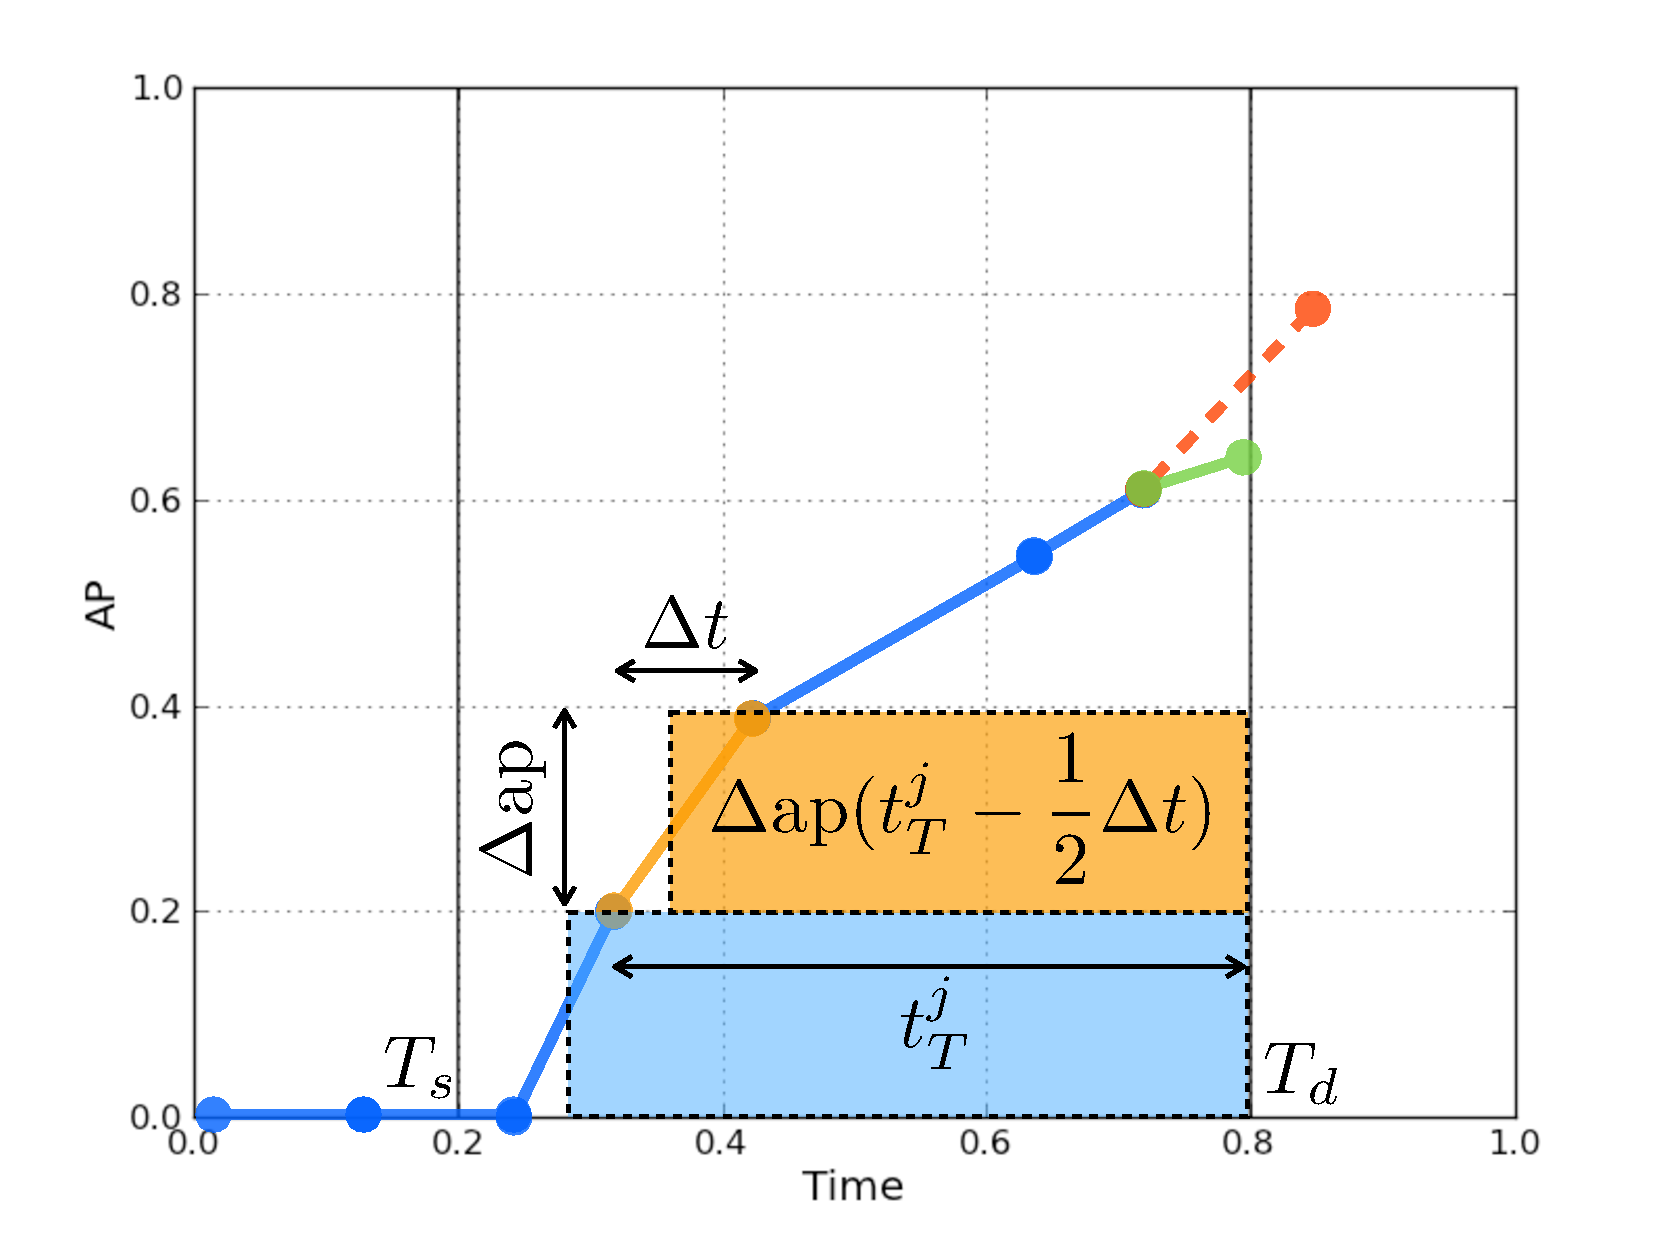
\includegraphics[width=\linewidth]{../../../2011-2012/figures/apvst_expl.pdf}
\caption{
Graphically representing our reward function.
}\label{fig:det_rewards}
\end{subfigure}
\begin{subfigure}[b]{.48\linewidth}
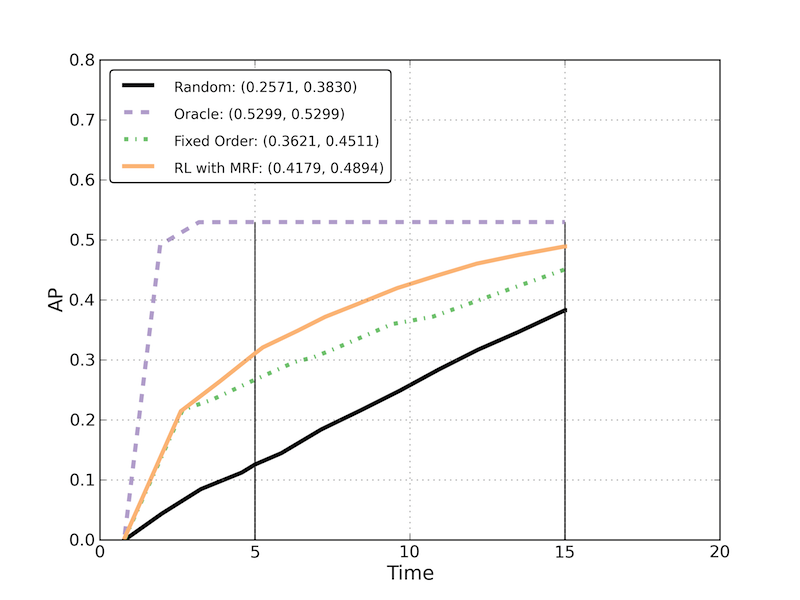
\includegraphics[width=\linewidth]{../../../2011-2012/figures/final1_515.png}
\caption{
AP vs. Time curves for Random, Oracle, the Fixed Order baseline, and our best-performing policy.
}\label{fig:results1}
\end{subfigure}
\end{figure}

We establish the first baseline for our system by selecting actions randomly at each step.
As shown in Figure~\autoref{fig:results1}, the \textbf{Random} policy results in a roughly linear gain of AP vs. time.
This is expected: the detectors are capable of obtaining a certain level of performance; if half the detectors are run, the expected performance level is half of the maximum level.

To establish an upper bound on performance, we plot the \textbf{Oracle} policy, obtained by re-ordering the actions at the end of each detection episode in the order of AP gains they produced.

We consider another baseline: selecting actions in a fixed order based on the value they bring to the AP vs. Time evaluation, which is roughly proportional to their occurrence probability.
We refer to this as \textbf{Fixed Order}.

Then there are instantiations of our method, as described in the previous section : \textbf{RL w/ Direct} inference and \textbf{RL w/ MRF} inference.
As the \textbf{MRF} model consistently outperformed \textbf{Direct} by a small margin, we report results for that model only.

In Figure~\autoref{fig:results1}, we can see that due to the dataset bias, the fixed-order policy performs well at first, as the person class is disproportionately likely to be in the image, but is significantly overtaken by our model as execution goes on and more rare classes have to be detected.

Lastly, we include an additional scene-level GIST feature that updates the posterior probabilities of all classes.
This is considered one action, and takes about $0.3$ seconds.
This setting always uses the MRF model to properly update the class probabilities with GIST observations.
This brings another small boost in performance.
The results are shown in \autoref{tab:results}.

Visualizing the learned weights in~\autoref{fig:weights}, we note that the GIST action is learned to never be taken in the greedy ($\gamma=0$) setting, but is learned to be taken with a higher value of $\gamma$.
It is additionally informative to consider the action trajectories of different policies in~\autoref{fig:trajectories}.

\begin{figure}[h!]
  \centering
  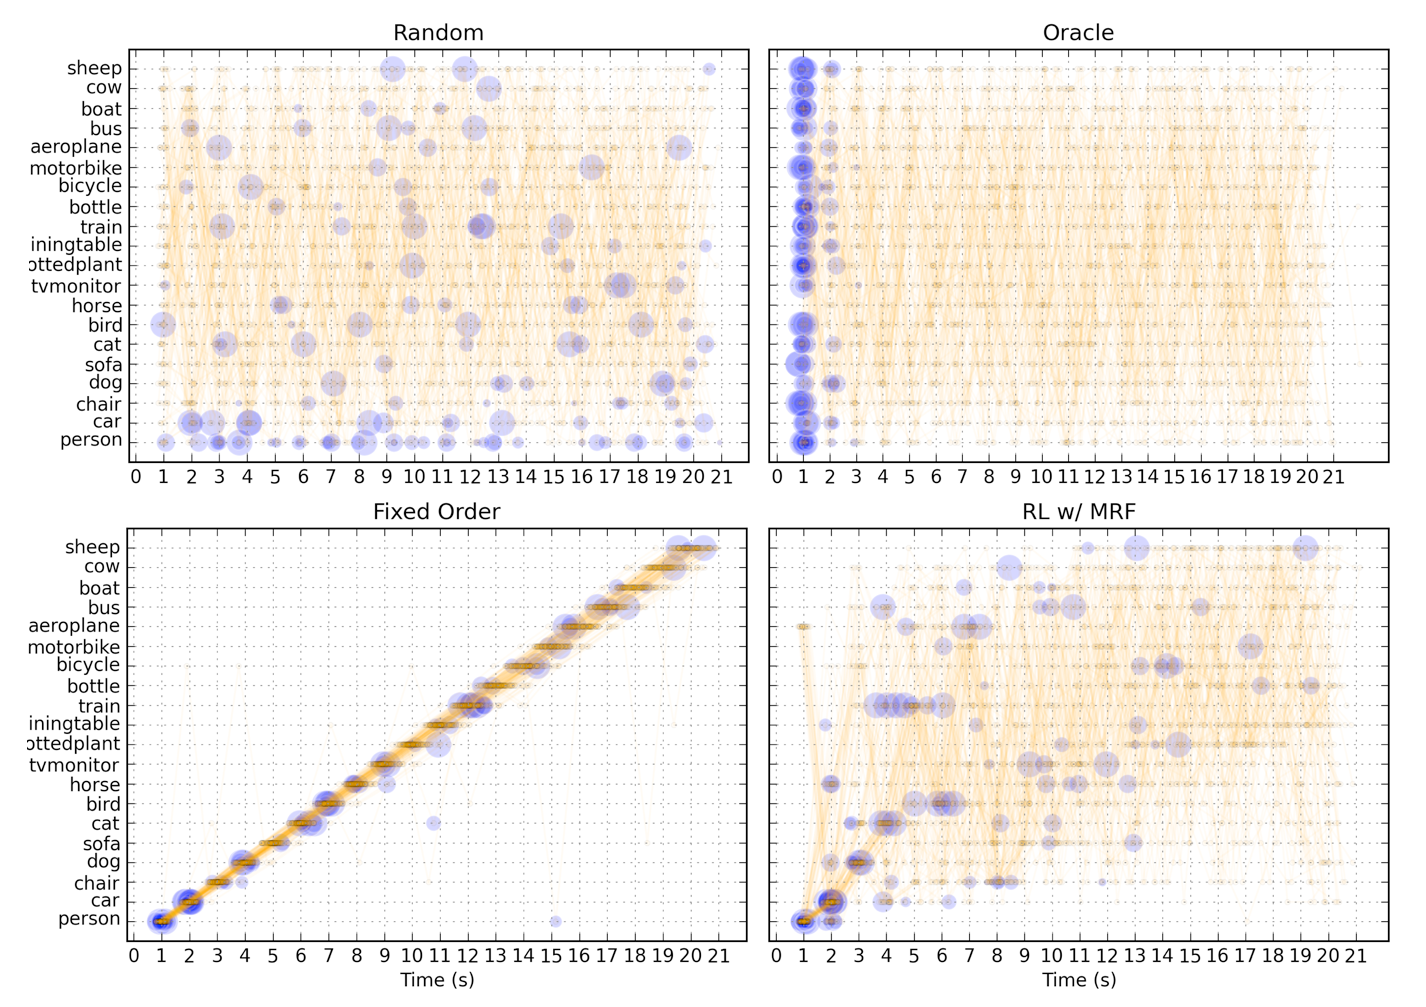
\includegraphics[width=0.85\linewidth]{../../../2011-2012/figures/trajectories.pdf}
  \caption{
Visualizing the action trajectories of different policies.
Action selection traces are plotted in orange over many episodes; the size of the blue circles correspond to the increase in AP obtained by the action.
We see that the \textbf{Random} policy selects actions and obtains rewards randomly, while the \textbf{Oracle} policy obtains all rewards in the first few actions.
The \textbf{Fixed Order} policy selects actions in a static optimal order.
Our policy does not stick a static order but selects actions dynamically to maximize the rewards obtained early on.
}
  \label{fig:trajectories}
\end{figure}

\begin{table}[t]
\caption{The areas under the AP vs. Time curve for different experimental conditions.}
\label{tab:results}
\begin{center}
\begin{tabular}{|c|c|c|c|c|c|}
\hline
Bounds & Random & Fixed Order & RL        & RL w/ GIST         & Oracle \\ \hline
(0,20) & 0.250  & 0.342       & 0.378     & \textbf{0.382}  & 0.488 \\
(0,10) & 0.119  & 0.240       & 0.266     & \textbf{0.267}  & 0.464 \\
(5,15) & 0.257  & 0.362       & 0.418     & \textbf{0.420}  & 0.530 \\ \hline
\end{tabular}
\end{center}
\end{table}
